%Texlive-full Version 3.141592-1.40.3 (Web2C 7.5.6)
%Kile Version 2.0.83


\documentclass[a4paper,10pt]{article}
\usepackage[utf8x]{inputenc}
\usepackage[T1]{fontenc} 

\usepackage{lmodern}
\usepackage[a4paper]{geometry}
%\usepackage[frenchb]{babel}
\usepackage{graphicx}
\usepackage{hyperref}

\usepackage{pstricks}
\usepackage{pst-node}
%\usepackage{wrapfig}
\usepackage{amsmath}
\usepackage{amsfonts}
\usepackage{amssymb}
\usepackage{textcomp}
%\usepackage{mathaccent}
\usepackage{listings}
\lstset{language=C++,basicstyle=\scriptsize \color{green},identifierstyle=\color{orange},keywordstyle=[1]\color{blue},columns=fullflexible,commentstyle=\textit}

\usepackage{color}



\begin{document}
%%%%%%%%%%%%%%%%%%   LOGO  %%%%%%%%%%%%%%%%%%%%%%%%%
\begin{center}
\rput(-4,1.5){\href{http://www.sofa-framework.org/}{
		\begin{tabular}{l}
		\resizebox{4cm}{0.6cm}{SOFA} \\ 
		\resizebox{6cm}{0.3cm}{Simulation Open Framework Architecture}
		\end{tabular}
		}
	    }
\end{center}
%%%%%%%%%%%%%%%%%%   LOGO  %%%%%%%%%%%%%%%%%%%%%%%%%

%%%%%%%%%%%%%%%%%% DOCUMENT TITLE %%%%%%%%%%%%%%%%%%%%%%%%% To be deleted when include in the global document
\vspace{1.5cm}
\begin{center}\resizebox{7cm}{0.6cm}{Adaptative Beam Plugin}\end{center}
%%%%%%%%%%%%%%%%%% DOCUMENT TITLE %%%%%%%%%%%%%%%%%%%%%%%%%

%%%%%%%%%%%%%%%%%%%%%%%%%%%%%%%%%%%%%%%%%%%%%%%%%%%%%%%%%%%%%%%%%%%%%%%%%%%%%%%%%%%%%%%%%
%=======================================================================================%
%%%%%%%%%%%%%%%%%%%%%%%%%%%%%%%%%%%%%%%%%%%%%%%%%%%%%%%%%%%%%%%%%%%%%%%%%%%%%%%%%%%%%%%%%
\section{Sofa Datatypes}
\subsection{RigidType}
\subsection{SolidType}

\section{Beam Element}
For the general introduction of beam theory and equations, see p.509~\cite{FEMBook2} .For detail of the construction local matrix, see the p.70 ~\cite{FEMBook1}.
\section{B-splines , B\'{e}zier Splines}
B-splines in general and B\'{e}zier splines in particulary can see in ~\cite{Bspline} or more detail in ~\cite{CourseGeo}. A spline tool can see at~\cite{SplineTool}. Here assumed several general formula. In general, a B\'{e}zier curve order $n$ is determined by $n+1$ control points (characteristic polygone) $P_{i,0 \leqslant i \leqslant n} $. Its trajectory is :
\[B(t) = \sum_{i=0}^n \hat{\textbf{B}} _{i,n}(t) . P_i   \]
Where $\hat{\textbf{B}} _{i,n}(t)$ are Bernstein polynomial given by 
\[\hat{\textbf{B}} _{i,n}(t) =  \complement_n^i .t^i.(1-t)^{n-i}  \]
The most usually used is the cubic B\'{e}zier , where trajectory is given by  
\[(1-t)^3.P_0    + 3.(1-t)^2 t.P_1    +   3.t^2(1-t).P_3   +  t^3.P_3\]
\begin{center}
 \begin{pspicture}(-5,-2)(5,2)
  \psline(-5,-2)(5,2)
    \pscurve(-4.5,-1.5)(-2,1)(2,1.5)(4,-1.5)
 \end{pspicture}
\end{center}

\section{Implementation }
\begin{center}
 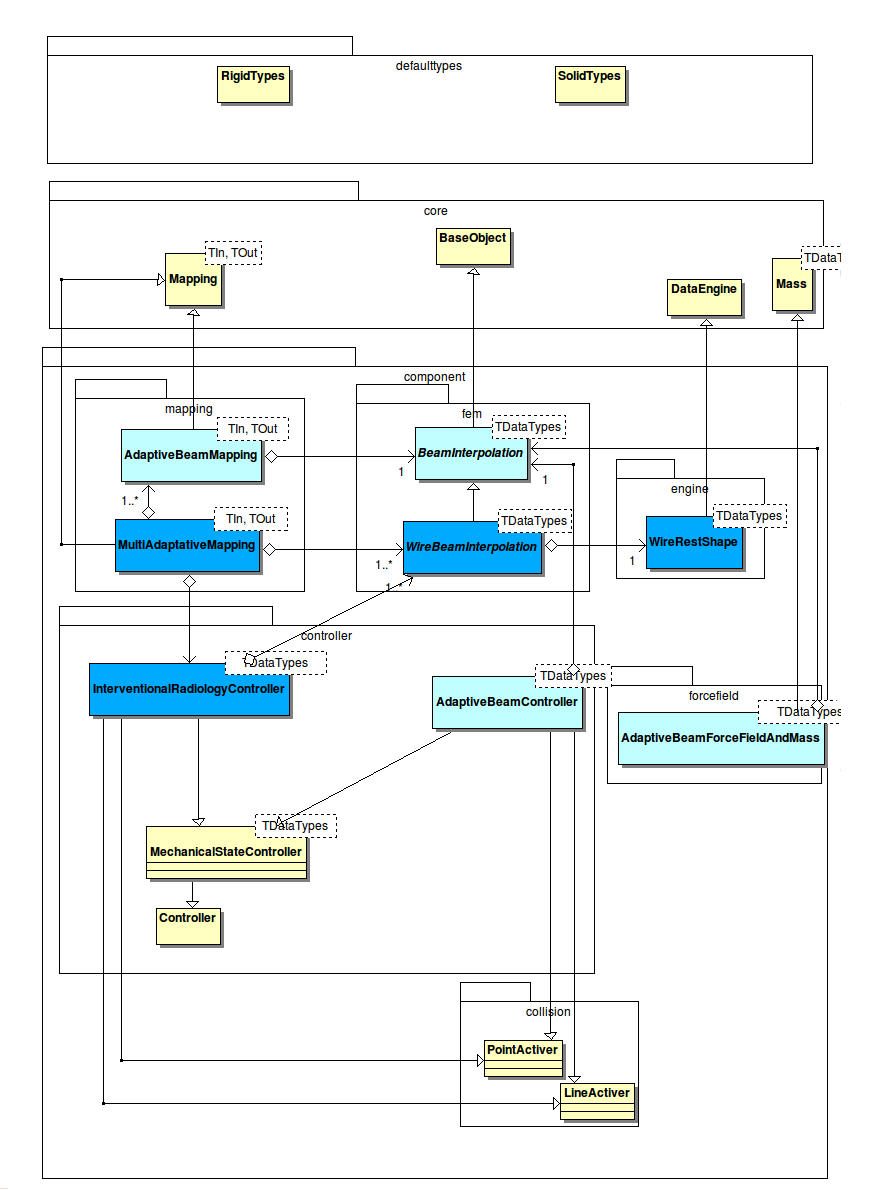
\includegraphics[scale=0.4]{UMLBeamAdapter}
\end{center}
\subsection{WireRestShape }
\subsection{BeamInterpolation }
\subsection{AdaptiveBeamForceFieldAndMass }
\subsection{AdaptiveBeamController }
\subsection{AdaptiveBeamMapping }
\subsection{WireBeamInterpolation }
\subsection{InterventionalRadiologyController }
\subsection{MultiAdaptiveMapping }
\bibliographystyle{siam}
\bibliography{AdaptativeBeam}
\end{document}